\documentclass[a4paper,12ptc]{jsarticle} %文字サイズは変えても良い
\usepackage[dvipdfmx]{graphicx}
\usepackage{amssymb, amsmath}
\usepackage{url}
\usepackage{tikz}  
\usetikzlibrary{decorations.pathreplacing,calligraphy}
\usepackage{float}
\usepackage{setspace}
\usepackage[top=30truemm,bottom=30truemm,left=25truemm,right=25truemm]{geometry} % ページの設定
\pagestyle{empty} %ページ番号なし
%\setlength{\headheight}{0truemm}
%\setlength{\parindent}{1zw}
\makeatletter
\def\section{\@startsection {section}{1}{\z@}{.7ex plus .2ex minus .2ex}{.1 ex plus 1.2ex}{\normalsize\bf}}
\makeatother
\setstretch{0.9}

\newcommand{\normal}{\mathcal{N}}
\newcommand{\exponential}{\mathcal{E}}
\newcommand{\truncnorm}{\mathcal{TN}}
\newcommand{\gam}{\mathcal{G}}
\newcommand{\C}{C}
\newcommand{\one}{1\!\!1}

\begin{document}
%\twocolumn[ 
\begin{center}
{\bf \Large 同時テンソル分解の拡張による医学データの統合}
\vspace{0.3em}
\begin{tabular}{rl}
\vspace{-0.1em} \bf 東京医科歯科大学難治疾患研究所 &  \bf 阿部興 \\
\vspace{-0.1em} \bf 名古屋大学大学院医学系研究科/東京医科歯科大学難治疾患研究所 &  \bf 島村徹平\\
\end{tabular}
\vspace{0.5em}
\end{center}
%]
\vspace{\baselineskip}

%\maketitle
\section{はじめに}
生命科学の分野においては, 生体内に存在する分子を網羅的に観測することが可能になった. 
これらは考察される対象の分子(これをモダリティと呼ぶことにする)が遺伝子であればゲノミクス,転写物であればトランスクリプトミクス,代謝物であればメタボロミクスといった様々な分野があり, 総称としてはオミクス(omics)データと呼ばれる. 中でも, ある1つのサンプルに対し複数のモダリティを計測するマルチオミクスデータは, 生命現象についての豊富な情報を持つものとして注目されている. 一方で, マルチオミクスデータをどのように分析すべきかは未だ議論が続いている.

複数のモダリティをまたいだ分析を難しくする原因の一つとして, 計測に関わる現実的な制約のために, 対応があるサンプルとないサンプルが混在する semi-paired なデータが多く見られることがあげられる. また, あるモダリティは計数データ, あるモダリティは連続値のデータといった形で, データの分布が大きく変わることも統一的な分析を難しくしている.

Abe \& Shimamura (2023) ではNMFを拡張し, 多次元のデータを柔軟に分析するモデルとして,  unified non-negative matrix factorization (UNMF) を提案した. しかし, UNMFはポアソン分布を仮定していたため, 本報告ではより幅広いクラスのデータを柔軟にあつかえる枠組みについて考察する.

%\section{}

\section{モデルと推定アルゴリズム}
\subsection{概要}
確率モデルとしての定式化の前に, まず我々が提案する手法の概要を, そのモチベーションが理解できるように述べたい. 簡単のため, 3階のテンソル $Y=(y_{i,j,k})$を考える. ここでは単に添字($i,j,k$)を定めたとき値が1つに決まるような変数(多次元配列)という意味でテンソルという語を用いる. さらに $\mathrm(vec)(Y)$ を適当な順番で $Y$ のすべての要素をベクトルに配置する作用素とする. 
CP分解(正準分解や並行因子分解とも呼ばれる)では各要素が次を満たすような行列 $V^{(k)}$ ($k=1,2,3$)を作る.
\begin{equation*}
y_{ijk} \approx \sum_{r}v_{ir}^{(1)} v_{jr}^{(2)} v_{kr}^{(3)}. 
\end{equation*}
この式は次のように書き換えられる:
\begin{equation}
y_{n} \approx \sum_{r}\prod_{d=1}^D v_{dr}^{x_{nd}} \label{eq_approx}
\end{equation}
ここで
\begin{align*}
V=(v_{dl})=\begin{pmatrix}
v^{(1)}\\
v^{(2)}\\
v^{(3)}
\end{pmatrix}
\end{align*}
and $x_{nd} \in \{0, 1\}$ is one-hot encoded matrix $(\xi_1, \xi_2, \xi_3)$. 
この表現は, 添え字の数が増えたり重複したり、欠損値が発生したりする場合でも矛盾なく扱える.
この定式化は図 \ref{fig_mosaic})に示す.

また交互作用項を考えることは
\begin{align*}
y_{ijk} &\approx \sum_{r}\prod_{d=1}^D v_{dr}^{x_{nd}} \\
&=\begin{cases}
\sum_{r}v_{ijr}^{(1)}v_{jr}^{(2)}v_{kr}^{(3)} & \mbox{when $X$ consisiting from $\xi_1 \cdot \xi_2$, $\xi_2$, and $\xi_3$}\\
\sum_{r}v_{ir}^{(1)} v_{jkr}^{(2)} v_{kr}^{(3)} & \mbox{when $X$ consisiting from $\xi_1$, $\xi_2 \cdot \xi_3$, and $\xi_3$}\\
\end{cases}
\end{align*}
このことも semi-paired なデータの分析にとって有益である. 例えば, 行の軸では対応があるが列の軸では対応のない行列を分析するときは, 列ダミーとモダリティの交互作用項を考える.

\begin{figure}
    \centering
    \begin{tabular}{c|c}
    \footnotesize (a)
    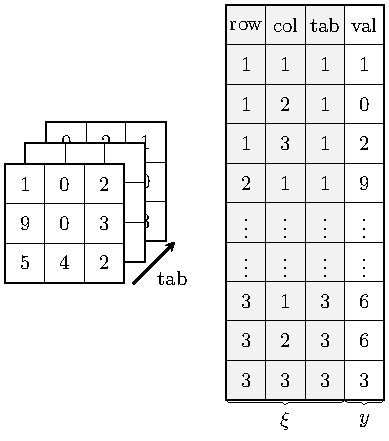
\includegraphics[width=0.2\textwidth]{img/threeway.pdf} &
    \footnotesize (b)
    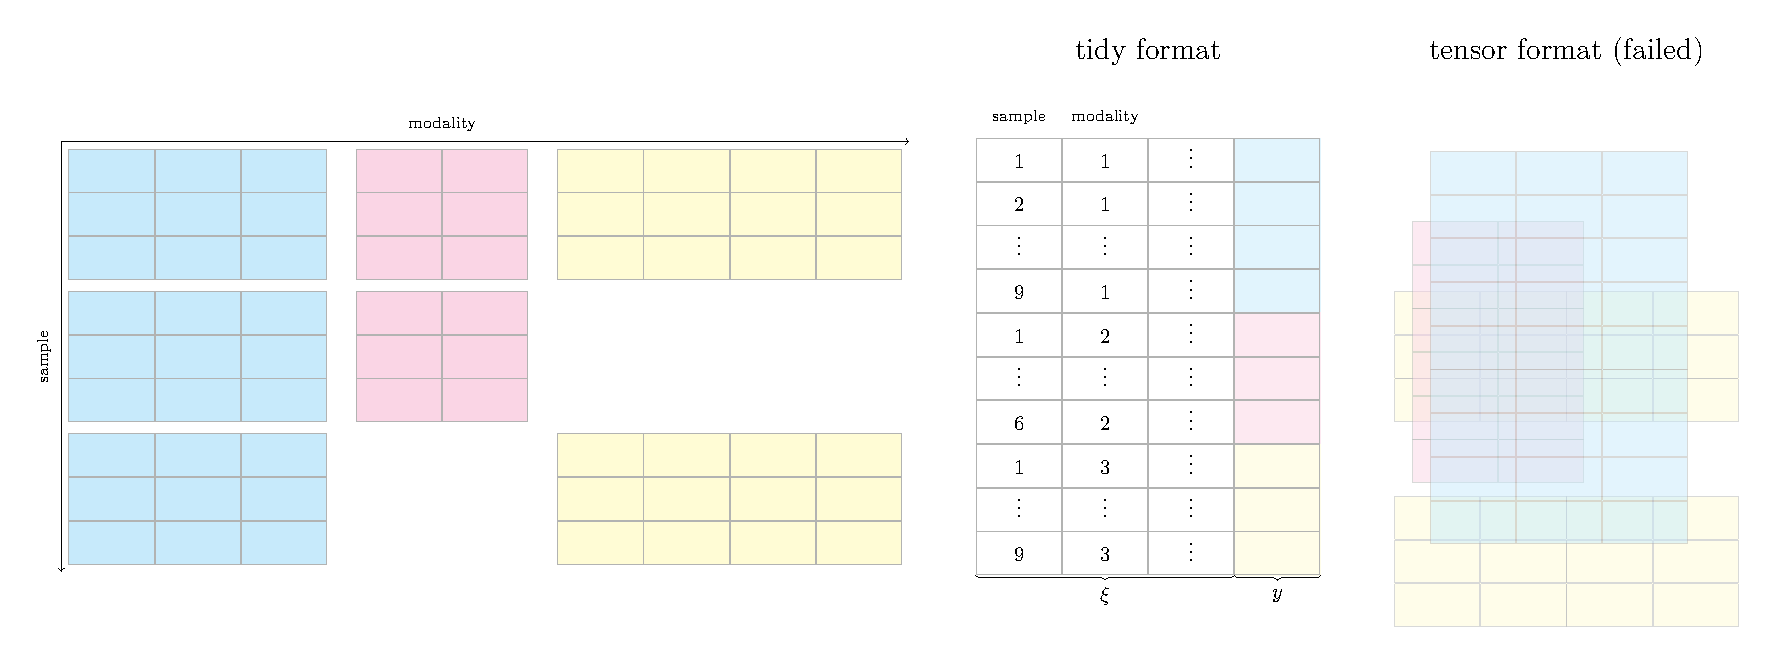
\includegraphics[width=0.7\textwidth]{img/mosaic.pdf} 
    \end{tabular}
    \caption{semi-pared なデータの統合. (a)多次元配列は右に示す形式(tidy-format)でも表現できる.  (b) 多次元配列の形式でまとめるのが難しいデータを tidy-formatで保管することもできる. ここで白いセルは欠測を意味する.}
    \label{fig_mosaic}
\end{figure}

\subsection{モデル}

\begin{align}
y_n &\sim \normal\left(y_n \mid \sum_{l=1}^L \prod_{d=1}^D v_{dl}^{x_{nd}}, \lambda^{-1}\right) \label{eq_mod1}\\
\lambda & \sim \gam(\lambda | a,b) \nonumber
\end{align}
ここで $V=(v_{dl})$ は $D \times L$  行列, $\gam(x|a,b)$ は形状パラメータとレートパラメータがそれぞれ $a$ と $b$のガンマ分布を表す.

$v_{dl}$ の事前分布については, 次のように非負制約の有無によって使い分ける:
\begin{align}
v_{dl} & \sim \normal(v_{dl} | 0,\tau^{-1}), \quad  \mbox{(非負のとき)} \label{eq_prior1}, \\
v_{dl} & \sim \truncnorm(v_{dl} | 0, \tau^{-1}), \quad  \mbox{(負の値を許すとき)} \label{eq_prior2}
\end{align}
ここで $\truncnorm(x | \mu, \sigma^2)$ は0で左側を切断された正規分布である.
この切断正規分布は次のように書ける:
\begin{equation*}
   \truncnorm(x | \mu, \sigma^2) \propto    \normal(x | \mu, \sigma^2) \one(x) 
\end{equation*}
ウェレここで $\one(x)$ は次の指標関数とした:
\begin{align*}
    \one(x)=\begin{cases} 1 & x>0\\
    0 &x \leq 0\end{cases}.
\end{align*}
非負制約の有無は$v_{d,l}$ごとに設定できるとしても, この節の議論に矛盾は生じないが, 我々の実装では第1引数で指定された変数のみに負の値を許すことにした. これは$1=(-1)\times(-1)$によって解釈が煩雑になるのを避けるためである.

\paragraph{中間変数}
次にモダリティによって $y$ の取りうる値の範囲が明確に変わる場合を考える.
例を上げると, データに負の値が生じないことが明らかなとき0を1と予測することと-1と予測することは対称に評価できない.
%観測モデルに正規分布を仮定することは当てはまりの誤差を左右対称に評価することを意味する.
そのため, 分布の台の変化に対応すべく, 次の中間的な変数 $z_n$を考える.
\begin{equation}
y_n = A(z_n), \quad z_n \sim \mathcal{N}\left(\sum_{l=1}^L \prod_{d=1}^Dv_{dl}^{x_{nd}}, \lambda^{-1}\right).
\end{equation}
関数 $A(x)$ 次のように選択する.
\begin{itemize}
\item $y_n$ が実数(連続)値をとるとき: 
$$
A(x)=x.
$$
\item $y_n$ が非負のとき:
$$
A(x)=\begin{cases}x, &x>0\\0 &x\leq 0\end{cases}.
$$
\item
$y_n$ が2値(0 or 1)のとき:
$$
A(x)=\one(x).
$$
\item
$y_n$ が非負の整数のとき:
$$
A(x)=\begin{cases}\lceil x\rceil, & x>0\\0 &x\leq 0\end{cases}.
$$
\end{itemize}

\paragraph{Multi-modal analysis} 
最後に付け加える変更は, 式\ref{eq_mod1} に示した観測モデルを次の 式\ref{eq_mod2}  に置き換えることである.
\begin{equation}
y_{n} = A_{m(n)}(z_{n}), \quad z_{n} \sim \mathcal{N}\left(\sum_{l=1}^L \prod_{d=1}^Dv_{dl}^{x_{ndm}}, \lambda^{-1}_m\right) \label{eq_mod2}    
\end{equation}
ここで、$m(n)$ はインデックス $n$ をモード $m(n)$ にマップする関数です。
複数のモードを考慮し、各モード $m$ の分布を変更したいと考えます。

\paragraph{対数同時密度}
ここまで述べたモデルに基づき $v_{dl}$ についての対数尤度関数 $\ell(v_{dl})$は次のように書ける:
\begin{align*}
& \ell(v_{dl}) =\sum_{n=1}^{N} \log p(z|V, X)\\
&= \sum_{n=1}^{N}\left(-\frac{\lambda}{2}\left\{ z_n -\sum_{l=1}^L\prod_{d=1}^D v_{dl}^{x_{nd}} \right\}^2\right)+ \C\\
&= -\sum_{m=1}^M\frac{h_{dlm}}{2}\left(v_{dl}^2-2v_{dl}\frac{\eta_{dlm}}{h_{dlm}}\right) +C,
\end{align*}
ここで $C$ は $v_{dl}$に依存しない定数, $\eta_{dl}$ と $h_{dl}$ は次のように置いた:
\begin{align}
\eta_{dlm} &= \sum_n x_{ndm} \prod_{d' \neq d} v_{dl}^{x_{ndm}}\left( z_{nm} - \sum_{l'\neq l} \prod_{d' \neq d} v_{dl}^{x_{ndm}} \right) \label{eq_eta}\\
h_{dlm} &= \sum_n \lambda_m x_{ndm} \prod_{d' \neq d} v_{dl}^{2x_{ndm}}. \label{eq_h}
\end{align}

\subsection{変分ベイズ法}
\label{est_sec}
この節では変分EMアルゴリズム\cite{Jordan}に基づき, 提案モデルについての推定量を導出する. 
本研究では平均場近似の仮定を置く. すなわち, 近似事後分布が互いに独立とした下でカルバックライブラ情報量の意味で事後分布を近似する$q(v_{dl})$ と $q(\lambda)$ を求める. また変分事後分布による$x$の期待値を $\langle x \rangle$ と表記する.
変分事後分布として,  次を得る.
\begin{align}
q(v_{dl})= \begin{cases}
\normal(\mu_{dl}, \sigma_{dl}) & \mbox{when the prior of $v_{dl}$ is not truncated} \\
\truncnorm(\mu_{dl}, \sigma_{dl}) & \mbox{when the prior of $v_{dl}$ is truncated},     
\end{cases} \label{qv}
\end{align}
ここで $\mu_{dl}$ と $\sigma_{dl}$ は次のように置いた:
\begin{align*}
\mu_{dl} &=\sum_{m=1}^M \frac{\langle \eta_{dlm} \rangle}{\langle h_{dlm}\rangle+\tau/\langle\lambda_m\rangle},\\
\sigma^2 &=\left(\tau + \sum_{m=1}^M \langle h_{dlm} \rangle \right)^{-1}.
\end{align*}
The variational posterior of $\lambda_{m}$ is,  
\begin{align}
    q(\lambda) = \gam\left(N_m/2 \eta_{dlm}, \left(\sum_m h_{dlm}+\tau\right)/2\right). \label{qlam}
\end{align}
変分ベイズ法の更新式で必要な各確率変数の期待値は次の通りである:
\begin{align*}
\langle v_{dl}\rangle &=\mu_{dl} + \sigma_{dl} \phi(-\mu_{dl}/\sigma_{dl})/\Phi(-\mu_{dl}/\sigma_{dl}),\\
\langle v_{dl}^2 \rangle&=\mu_{dl}^2 + \sigma_{dl}^2 + \mu_{dl} \sigma_{dl} \phi(-\mu_{dl}/\sigma_{dl})/\Phi(-\mu_{dl}/\sigma_{dl}),\\
\langle \lambda_m \rangle &= (N_m \langle \eta_{dlm} \rangle ) / \left(\sum_m \langle h_{dlm} \rangle +\tau\right).
\end{align*}
ここで $\phi(x)$ と $\Phi(x)$ をそれぞれ標準正規分布の確率密度関数, 分布関数とした.

潜在変数 $z_n$, についての期待値はMonte-Carlo積分で評価する.すなわち,$\tilde z_n$ を次のように変分事後分布から疑似乱数でサンプルする:
\begin{itemize}
\item Rectified
\begin{align}
q(-z_n) = \begin{cases}
    \mathcal{TN}(-z_n|-f_n, \sigma_n^2) & y_n=0,\\
    z_n = y_n \mbox{~with probability 1} & y_n>0
\end{cases}
\end{align}
\item Binary
\begin{align}
q(-z_n) = \begin{cases}
    \mathcal{TN}(-z_n|-f_n, \sigma_n^2) & y_n=0,\\
    \mathcal{TN}(z_n|f_n, \sigma_n^2) & y_n=1
\end{cases}
\end{align}
\end{itemize}

要約すると, 近似事後分布を実現するアルゴリズムは次のようになる:
\begin{itemize}
\item 変分 E-ステップ: $\tilde{z}_n$ をサンプルする 
\item 変分 M-ステップ:  式\ref{qv} を用いて$q(v_{dl})$ を, 式\ref{qlam} を用いて$q(\lambda)$を更新する. 
\end{itemize}

当日は推定量を評価するシミュレーションにデータ分析事例をあわせて報告する.

\begin{thebibliography}{9}
\bibitem{AbeShimamura} Abe K \& Shimamura T. (2023). UNMF: A unified non-negative matrix factorization for multi-dimensional omics data. {\em Briefings in Bioinformatics.}  24 (5), bbad253.
\bibitem{Jordan} Jordan~MI, Ghahramani~Z, Jaakkola~TS \& Saul~LK. (1999). An introduction to variational methods for graphical models. {\em Machine learning}, 37(2), 183-233.
\end{thebibliography}
\end{document}  m 